
% ISA Documentation
% Martin Benes
% FIT VUT
% 2018/2019

% ---------------------------- HEADER ---------------------------- %
\documentclass[10pt,a4paper,titlepage]{article}

% packages
\usepackage[english]{babel}
\usepackage[utf8]{inputenc}
\usepackage[margin=100pt]{geometry} 
\usepackage{graphicx}   % Import pictures
\usepackage{caption}
\usepackage[backend=biber, sorting=none]{biblatex}

% references (BiBTeX)
\addbibresource{manual.bib}   



% --------------------------- BODY ----------------------------- %
\begin{document}
    

    % ----------------- Title Page -------------------%
    \begin{titlepage}
    \begin{center}
        % Headings
        \textsc{\LARGE Brno University of technology}\\[0.5cm]
        \textsc{\large Faculty of Information Technology}\\[8cm]
    
        % Title - lines
        { \huge \bfseries Monitoring and Generating Tools of Simple Distance-Vector Protocols}\\[0.3cm]
        { \Large \bfseries Project documentation}\\[0.5cm]
        { \bfseries Martin Benes}\\
    
    \end{center} 
    \end{titlepage}
    \newpage
    

    % ------------- Table of Contents ----------------%
    \tableofcontents
    \newpage





    % -------------------- Content ----------------------%
    \section{Introduction}
        \subsection{Task}
            The task of the project was to gather informations about RIP protocols, RIPv1, RIPv2 and RIPng and
            to write two programs in C, one of them RIP sniffer and the other RIP fake responder.

        \subsection{Motivation}
            Internet. It is everywhere nowadays - it helps us order pizza, find a taxi, do shopping,
            connect us with all our friends but it also controls the lights, air condition units etc;
            it has become a significant part of our lives. There is a lot of data flowing through each
            its part in every moment. This dataflow is directed ({\it routed}) by devices called routers,
            knots in the huge network.

            \begin{figure}[h!]
                \begin{center}
                    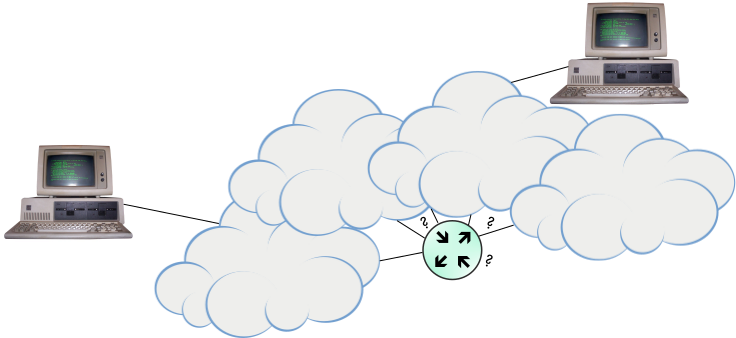
\includegraphics[width=0.80\textwidth]{routing.png}
                    \caption{ Routing. \label{fig:routing} \cite{Cloudimage} \cite{PCimage}}
                \end{center}
            \end{figure}

            Each router has multiple routes connected to it and it has a single task: it recieves
            a chunk of data (packet) with an address on it and it is supposed to send it closer to
            the target device in the network as you can see in the figure \ref{fig:routing}.
            The router must decide which route should the packet go. And this is exactly what the
            RIP protocol does. 
    



    \section{RIP Protocol}
        {\it Routing Information Protocol} is a routing protocol. It enables routers to communicate and to react
        on the network topology changes. RIP is a distance-vector protocol - no router knows the whole structure
        of the network. The method it uses to count the shortest path is Bellman-Ford algorithm. A hop count
        is used as a path cost.


        \subsection{Messages}
            The protocol uses UDP transport protocol and it has registered port 520 (RIPv1, RIPv2) and 521 (RIPng).
            Two basic types of messages are used, RIP Request and RIP Response.
            \paragraph{RIP Request}
                RIP Request is sent when the router asks other router for the routing table content (all or just a part).
            \paragraph{RIP Response} 
                RIP Response includes the routing table of the sender. The destination port is the port in the Source Port
                array in the RIP Request. But it can be sent even without previous RIP Request received.


        \subsection{Communication}
            A newly connected router broadcasts a RIP Request to all interfaces. All the routers running RIP
            respond sending RIP Response packet containing their routing tables. The router will calculate its own.
            This process is shown in the figure \ref{fig:RIPstart}.

            \begin{figure}[h!]
                \begin{center}
                    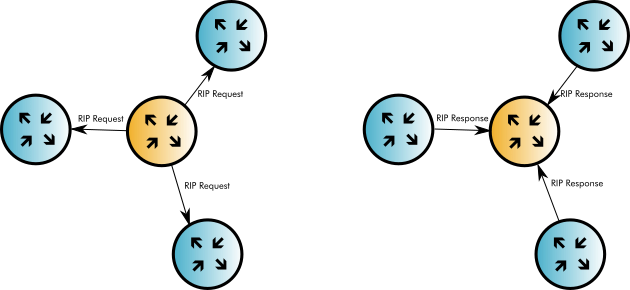
\includegraphics[width=0.70\textwidth]{RIPstart.png}
                    \caption{Initialization Process of RIP Protocol. \label{fig:RIPstart}}
                \end{center}
            \end{figure}

            Then the router can route all the packets coming through. Every route is supposed to regularly broadcast an update,
            its frequence is set by standard to 30 s. If the update in form of RIP Response comes, the timer will be reset, if not,
            the route is marked as invalid, the graph is to be seen in the figure \ref{fig:RIPupdate}. After that, "garbage collector timer"
            120~s is set for that route and after that the route is removed from the routing table. 

            \begin{figure}[h!]
                \begin{center}
                    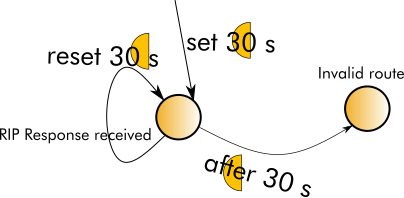
\includegraphics[width=0.60\textwidth]{RIPupdate.png}
                    \caption{Update Process of RIP Protocol. \label{fig:RIPupdate}}
                \end{center}
            \end{figure}

            If the router detects a change, either an unavailable interface or a new connected neighbor, the triggered update is made. The
            router broadcast the change using RIP Response packets to all it interfaces. The change is then spread by all routers through
            the network. This process is described in the figure \ref{fig:RIPtriggered}.

            \begin{figure}[h!]
                \begin{center}
                    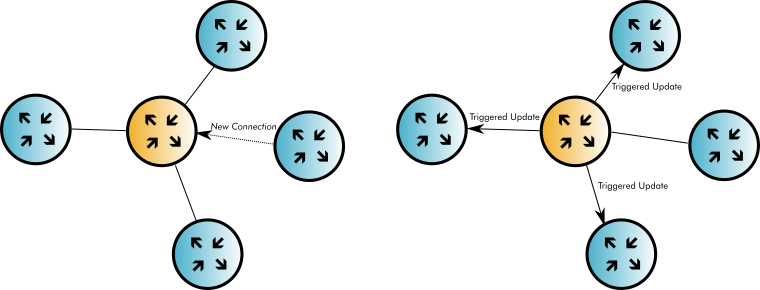
\includegraphics[width=0.75\textwidth]{RIPtriggered.png}
                    \caption{Triggered Update Process of RIP Protocol. \label{fig:RIPtriggered}}
                \end{center}
            \end{figure}


        \subsection{Route Determination}
            Three main items of each record in the routing table are address of the network/station, distance (hops)
            and network interface ID. RIP protocol enables routers to share their routing tables and make sending of data through
            the network much more efficient. The receiving router always compares the new information with the one he has.

            If the network X is reachable in N+1 hops (router increases the number by one), it is compared with the content
            of the routing table. If the new route is better, it is set and algorithm is propagated to the neighbors to
            recalculate - this is done again again until the algorithm reaches convergence.


        \subsection{Versions}
            \paragraph{RIPv1}
                Standardized by RFC 1058 (1988) works for routing IPv4 addresses of A, B and C classes. There is no support for
                network masks (CIDR) - all the networks must have the same mask. A mutual authentication of routers is also not
                possible, it must be done by different layer. The structure of RIPv1 header and all the packet headers is to be
                seen in the figures \ref{fig:RIPheader} and \ref{fig:RIPheader}.\cite{RFC1058}
            \paragraph{RIPv2}
                The RFC 1388 (1993) introduced the second version of protocol. Some issues were solved, an effort for keeping
                a backward compatibility caused that RIPv2 let most of the problems of its predecessor stay. The protocol
                enabled CIDR, as same as the mutual authentication, where MD5 is used. The passwords are sent not encrypted,
                so it can be very easily attacked. Communication was changed from broadcast to multicast. New route tags
                provides distinction between routes found by RIP and the routes from different protocols. Headers of the packet
                with RIPv2 are the same as RIPv1 (figure \ref{fig:RIPheaders}). You can see a RIPv2 header structure in the figure
                \ref{fig:RIPheader}. If there is a difference, the RIPv2 is in the parentheses. \cite{RFC2453}

                \begin{figure}[h!]
                    \begin{center}
                        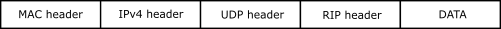
\includegraphics[width=0.65\textwidth]{rip_hs.png}
                        \caption{RIPv1 and RIPv2 protocol packet. \label{fig:RIPheaders}}
                    \end{center}
                \end{figure}

                \begin{figure}[h!]
                    \begin{center}
                        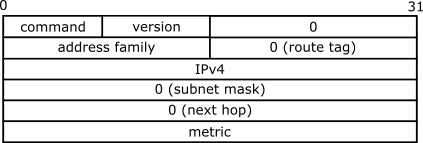
\includegraphics[width=0.60\textwidth]{rip_h.png}
                        \caption{RIPv1 (RIPv2) header. {\it RIPv2 item is either the same or in parentheses}. \label{fig:RIPheader}}
                    \end{center}
                \end{figure}

            \paragraph{RIPng}
                The RFC 2080 (1997) is a reaction to IPv6. Except of that, it erased support of encryption, that must be covered
                by IPsec. The structure of packet in the figure \ref{fig:RIPheaders} stays the same as previous versions,
                RIPng header is shown in the figure \ref{fig:RIPngheader}.
                \cite{RFC2080} \cite{RFC2081}

                \begin{figure}[h!]
                    \begin{center}
                        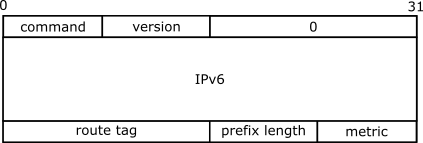
\includegraphics[width=0.50\textwidth]{ripng_h.png}
                        \caption{RIPng header. \label{fig:RIPngheader}}
                    \end{center}
                \end{figure}

        \subsection{Problems}
            The popularity of the protocol is caused by its simplicity. Although it has some issues which led into replacing
            RIP protocol in different routing protocols (EIGTP, OSPF).
            \paragraph{Slow Convergence}
                Due to the fact that timeout for sending RIP Response is set by RFC to 30~s, convergence of the whole algorithm
                might take minutes, which is ages for today networing. The propagation of failure is even 180~s, initial delay
                for propagation. At the networks of hundreds of routers, the time of convergence will become intolerable and
                the RIP protocol is useless there.
            \paragraph{Max hop count}
                The max hop count is limited to 15 - longer paths are not possible, because hop count 16 means unreachable network
                (distance is infinity). Also, hop count does not always have to be the best metric. It might be better to use delay,
                load or reliability.
            \paragraph{Unsupported CIDR and IPv6}
                The first version of protocol was not designed for classless addresses and IPv6; The CIDR is possible in RIPv2
                and special protocol RIPng was designed for IPv6 support. 
        
        \subsection{Optimalizations}
            During each update, RIP floods the network with a lot of traffic. Therefore there are techniques that makes this procedure
            more efficient.
            \paragraph{Split Horizon}
                When the router finds a better route, it is sent to all his neighbors. When Split Horizon is used, the update is
                not sent to the router that sent us the better route at the first place.
            \paragraph{Poison Reverse} 
                When the router finds out that some route is unreachable, it immediately updates all its neighbors. \cite{RIPJuniper}
                \cite{RIPGuide} \cite{RIPWikipedia} \cite{computernetworking} \cite{mistrovstvivsitich}
    
    \newpage
    \section{Implementation}

        \subsection{Sniffer}
        
            % program description
            % process of work
            
        \subsection{Fake Responder}
        
            % program description
            % process of work
    
    
    \section{Application}
        
        \subsection{Testing System Structure}
            System where the programs were tested had following structure: virtualized Linux Mint on the parent Windows 10. VirtualBox
            was used as the virtualization engine. As you can see in the figure \ref{fig:VBWinMint}, there are two interfaces. One of them
            is set to NAT, it is called {\it enp0s3} in the virtualized Linux Mint. The other called {\it enp0s8} in Linux is host only.
            It is used for the program to listen to.

            Inside the Linux Mint there is another VirtualBox installed, which virtualizes FreeBSD used for creating the RIP traffic.
            All the traffic from the FreeBSD is bridged to the enp0s8 where the sniffer may work with it. You can see the settings
            in the figure \ref{fig:VBMintBSD}.

            \begin{figure}[h!]
                \begin{center}
                    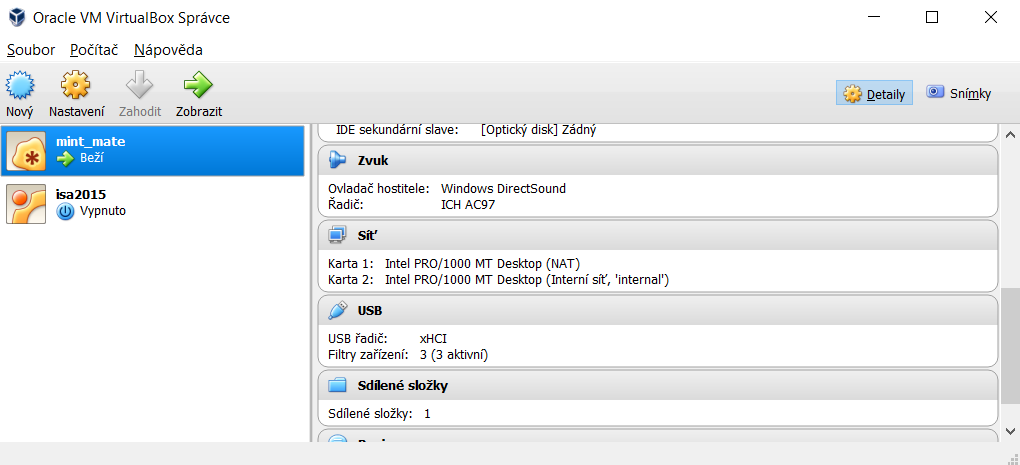
\includegraphics[width=0.50\textwidth]{winmint.png}
                    \caption{Settings of virtualized Linux Mint in VirtualBox on Windows. \label{fig:VBWinMint}}
                \end{center}
            \end{figure}

            \begin{figure}[h!]
                \begin{center}
                    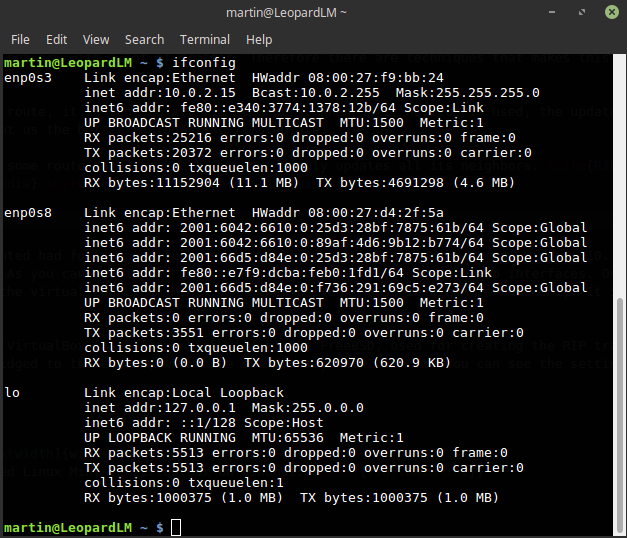
\includegraphics[width=0.50\textwidth]{mintifconfig.png}
                    \caption{Interfaces on Linux Mint. \label{fig:MintIfconfig}}
                \end{center}
            \end{figure}

            \begin{figure}[h!]
                \begin{center}
                    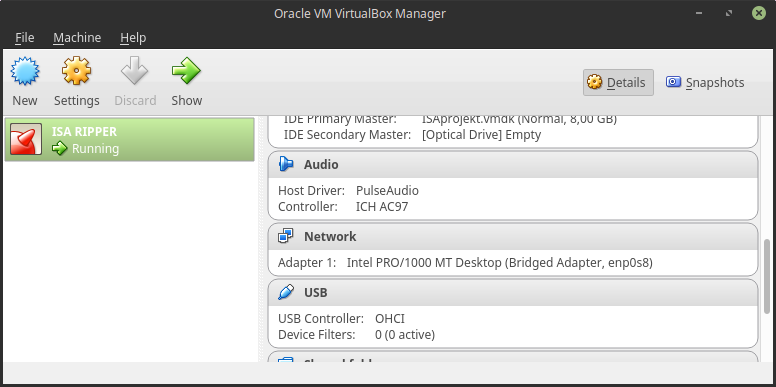
\includegraphics[width=0.50\textwidth]{mintbsd.png}
                    \caption{Settings of virtualized FreeBSD in VirtualBox on Linux Mint. \label{fig:VBMintBSD}}
                \end{center}
            \end{figure}

            \begin{figure}[h!]
                \begin{center}
                    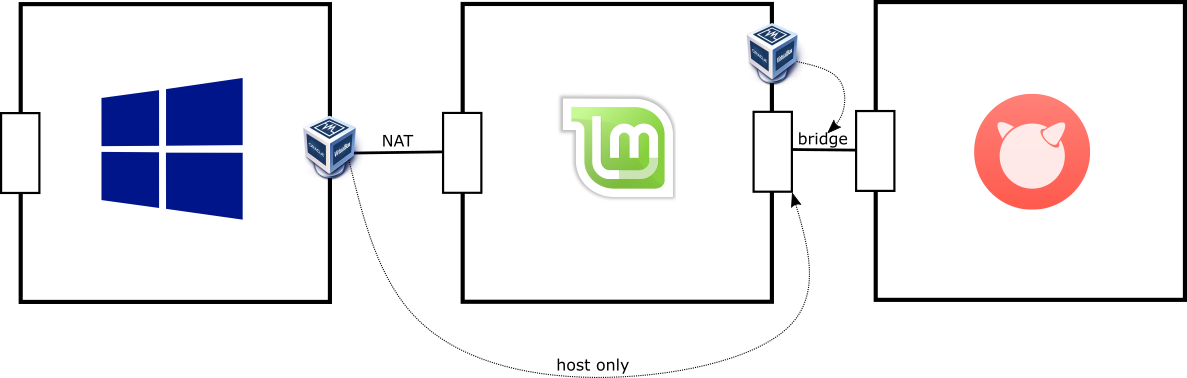
\includegraphics[width=0.80\textwidth]{programming.png}
                    \caption{Structure of the whole testing system. \label{fig:TestingSystem} \cite{WindowsLogo} \cite{MintLogo} \cite{FreeBSDLogo} \cite{VirtualBoxLogo}}
                \end{center}
            \end{figure}

        \subsection{Testing}
            % description of testing
            % figure with printscreens from Wireshark
    
    \newpage
    \printbibliography
    
    \end{document}